\subsection{Сценарий 4: Simple Tag}

Как уже упоминалось \hyperref[exp-st]{выше}, этот сценарий не подразумевает коммуникационных действий. Но он был выбран нами, так как он достаточно сложный, и при этом агенты из одной команды имеют одинаковые пространства наблюдения и действий, что позволяет применить вариант алгоритма MADDPG с общим мозгом.

\subsubsection{Двое против одного}

Был поставлен эксперимент с двумя преследователями и одной жертвой.

На \firef{fig-st-reward-ad} и \firef{fig-result-st-reward-ag} изображены графики средней награды преследователей и жертв. Видно, что графики симметричны. Когда преследователи выучиваются двигаться в нужном направлении и понимают, что нужно преследовать жертву, они получают большую награду, а жертва~--- меньшую. После чего жертва выучивается убегать от преследователей~--- тогда её награда растёт, а награда преследователей снижается. Так же, как и в \hyperref[exp-results-svc]{предыдущем сценарии}.

\begin{figure}[!htbp]
    \adjustbox{minipage=1.3em,valign=t}{\subcaption{}\label{fig-st-reward-ad}}%
    \begin{subfigure}[t]{\dimexpr.5\linewidth-1.3em\relax} %разрешили выделить 0,5 стр в ширину на рисунок
        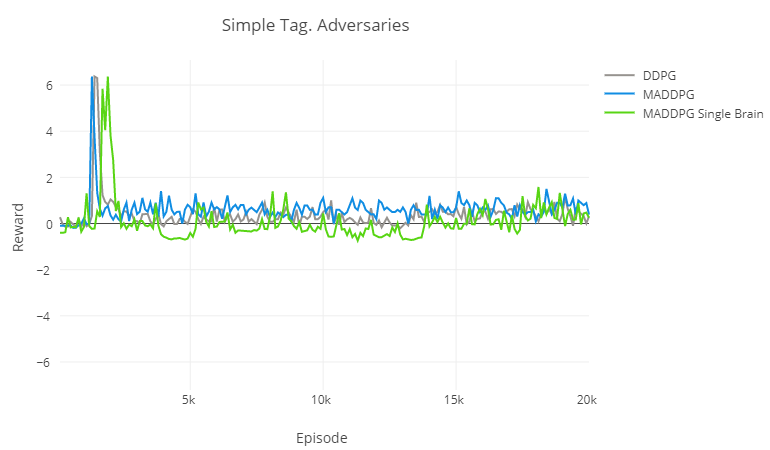
\includegraphics[height=0.19\textheight,valign=t]{my_folder/images/ch5/st-reward-ad.png} %высоту рисунка выставили как 0,3 от высоты наборного поля
    \end{subfigure}
    %	\hfill %выровнять по ширине
    \adjustbox{minipage=1.3em,valign=t}{\subcaption{}\label{fig-result-st-reward-ag}}%
    \begin{subfigure}[t]{\dimexpr.5\linewidth-1.3em\relax}%разрешили выделить 0,5 стр в ширину на рисунок
        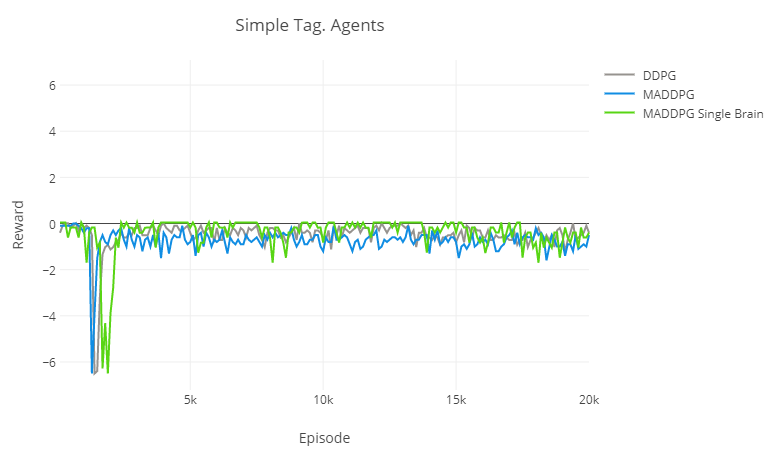
\includegraphics[height=0.19\textheight,valign=t]{my_folder/images/ch5/st-reward-ag.png}%высоту рисунка выставили как 0,3 от высоты наборного поля
    \end{subfigure}
    \captionsetup{justification=centering} %центрировать
    \caption{Награда с применением алгоритма DDPG, MADDPG, MADDPG с общим мозгом: {\itshape a}~--- преследователей; {\itshape b}~--- жертв}\label{fig:spbpu_main_bld-two-photos}
\end{figure}

В \taref{tab-st-time} указано время, затраченное на обучение в данной конфигурации для разных алгоритмов.

\begin{table}[t!]
    \centering\small
    \caption{Среднее время, потраченное на обучение с различными алгоритмами в 20000 эпизодах: 2 преследователя, 1 жертва}
    \label{tab-st-time}
    \begin{tabular}{|l|l|l|l|l|l|}
        \hline
        & DDPG               & MADDPG             & MADDPG с одним мозгом \\
        \hline
        Время, 20000 эпизодов & 27960 $\pm$ 2236~с & 37430 $\pm$ 2994~c & 13320 $\pm$ 1065~c    \\ \hline
    \end{tabular}
    \normalsize% возвращаем шрифт к нормальному
\end{table}

\subsubsection{Четверо против двоих.}

С этим сценарием также были поставлены эксперименты с более сложными настройками~--- 4 преследователя и 2 жертвы.

\begin{figure}[!htbp]
    \adjustbox{minipage=1.3em,valign=t}{\subcaption{}\label{fig-result-st-4vs2-ddpg}}%
    \begin{subfigure}[t]{\dimexpr.5\linewidth-1.3em\relax} %разрешили выделить 0,5 стр в ширину на рисунок
        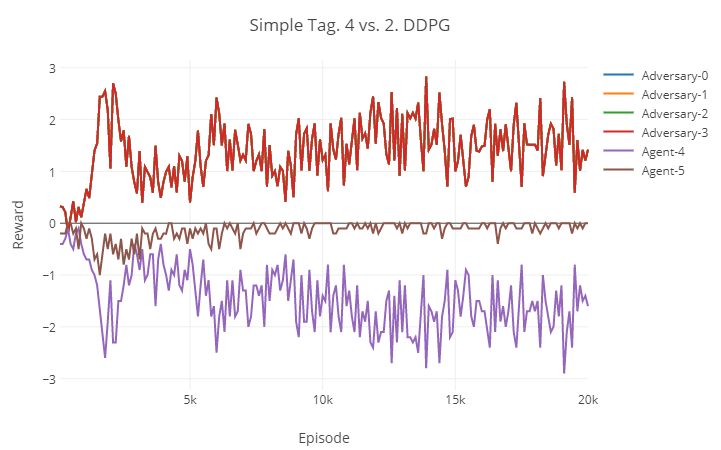
\includegraphics[height=0.20\textheight,valign=t]{my_folder/images/ch5/st-4vs2-ddpg.png} %высоту рисунка выставили как 0,3 от высоты наборного поля
    \end{subfigure}
    %	\hfill %выровнять по ширине
    \adjustbox{minipage=1.3em,valign=t}{\subcaption{}\label{fig-result-st-4vs2-maddpg}}%
    \begin{subfigure}[t]{\dimexpr.5\linewidth-1.3em\relax}%разрешили выделить 0,5 стр в ширину на рисунок
        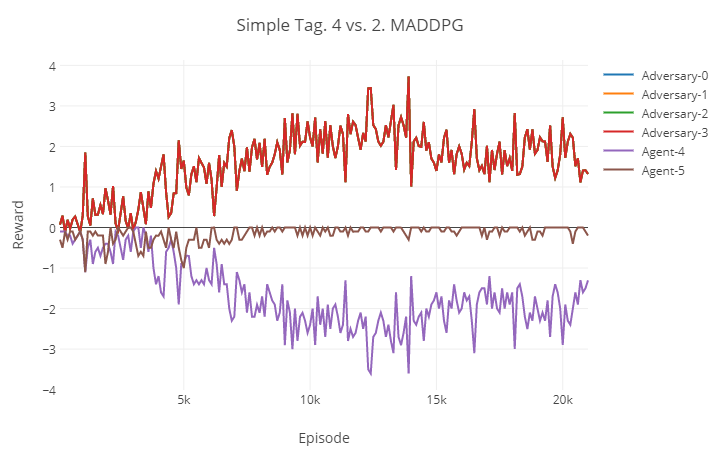
\includegraphics[height=0.20\textheight,valign=t]{my_folder/images/ch5/st-4vs2-maddpg.png}%высоту рисунка выставили как 0,3 от высоты наборного поля
    \end{subfigure}
    \adjustbox{minipage=1.3em,valign=t}{\subcaption{}\label{fig-result-st-4vs2-maddpg-sb}}%
    \begin{subfigure}[t]{\dimexpr.5\linewidth-1.3em\relax}%разрешили выделить 0,5 стр в ширину на рисунок
        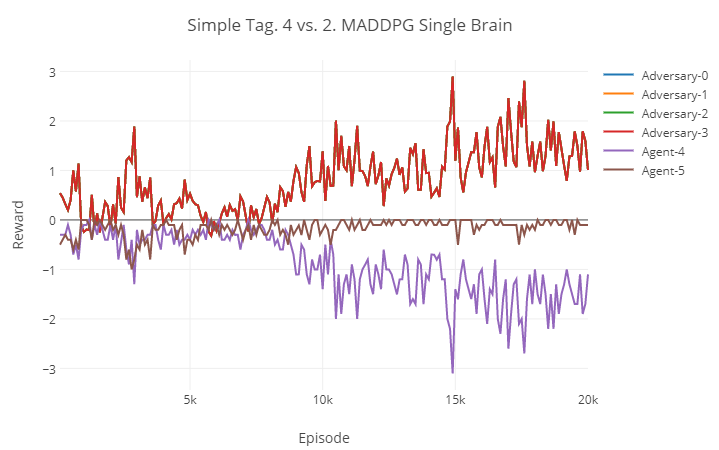
\includegraphics[height=0.20\textheight,valign=t]{my_folder/images/ch5/st-4vs2-maddpg-sb.png}%высоту рисунка выставили как 0,3 от высоты наборного поля
    \end{subfigure}
    \captionsetup{justification=centering} %центрировать
    \caption{Награда каждого из 6 агентов с применением алгоритма: {\itshape a}~--- DDPG; {\itshape b}~--- MADDPG; {\itshape c}~--- MADDPG с общим мозгом}\label{fig:spbpu_main_bld-two-photos}
\end{figure}

На \firef{fig-result-st-4vs2-ddpg}, \firef{fig-result-st-4vs2-maddpg} и \firef{fig-result-st-4vs2-maddpg-sb} изображены графики средней награды преследователей и жертв.

В \taref{tab-st-4vs2-time} указано время, затраченное на обучение в данной конфигурации для разных алгоритмов.

\begin{table}[t!]
    \centering\small
    \caption{Среднее время, потраченное на обучение с различными алгоритмами в 20000 эпизодах: 4 преследователя, 2 жертвы}
    \label{tab-st-4vs2-time}
    \begin{tabular}{|l|l|l|l|l|l|}
        \hline
        & DDPG               & MADDPG             & MADDPG с одним мозгом \\
        \hline
        Время, 20000 эпизодов & 40980 $\pm$ 3278~с & 60480 $\pm$ 4838~с & 31100 $\pm$ 2488~с    \\ \hline
    \end{tabular}
    \normalsize% возвращаем шрифт к нормальному
\end{table}

\subsubsection{Вывод из результатов эксперимента.}

Как уже упоминалось выше, награды преследователей и жертв симметрично-противоположны. Это вытекает из того, что: во-первых~--- сам сценарий имеет конкурентную природу, а награда одним агентам даётся за то же, за что у других отнимается (это описано в разделе \hyperref[intro-st]{Вводная глава: Сценарий 4. Simple Tag}); во-вторых~--- во время тренировки обучаются как преследователи, так и жертвы.

Если взять обученную модель агента одной из команд и начать тренировать против него агентов другой команды, но при этом не обучать первого агента, можно было бы увидеть некоторой прогресс, увидеть на графике, как награда первого агента со временем снижается, а его противников~--- растёт.

Приведённые выше графики наград отчётливо это показывают. В ходе обучения они ни к чему не сходятся.

Однако, это не значит, что агенты не обучаются. При запуске игры на обученных моделях видно, что агенты из обеих команд ведут себя вполне адекватно~--- преследователи гоняются за жертвами, жертвы избегают преследователей. Как на правом скриншоте на \firef{fig:st}.

И это не помешало нам измерить затраченное время на выполнение каждого эксперимента.

Из \taref{tab-st-time} и \taref{tab-st-4vs2-time} видно, что алгоритм DDPG показал лучшие результаты, чем MADDPG. Это объясняется тем, что этот алгоритм проще и требует меньших вычислительных мощностей, в то же время, он не даёт тех возможностей коммуникации, которые могут быть необходимы во многих задачах.

Зато алгоритм MADDPG с общим мозгом показал значительное преимущество. Это объясняется тем, что в этом случае не происходит обучения одному и тому же разных наборов сетей актора-критика. Обучается один <<мозг>> для каждой команды агентов.
